
\section{Introduction}

This chapter introduces three new methods to detect synaptic connections from voltage signals.

The first two methods are still based on the STA (spike-triggered average), as in \cref{ch3-STA}. And, also as before, they still use shuffled presynaptic spiketrains\footnote{
    A note on terminology: when we write `presynaptic' or `postsynaptic' in this thesis, we often mean the neuron that we are testing as a \emph{possible} presynaptic / postsynaptic connection.
}
to provide a null-distribution for the test statistic

The difference is in how the STA is used. In \cref{ch3-STA} we used the height of the STA (`peak-to-peak', ptp) as a test statistic.\\
The first new method here instead \emph{correlates} the STA with some template of what the STA of a true connection would look like, to calculate a test statistic.\\
The second method fits an idealized function to the STA, and uses the goodness-of-fit as a test statistic.

The third method steps away entirely from the STA, and instead uses the data of the different spike-triggered windows directly, without averaging them together in an STA.

As the focus was on comparing these new methods with each other and with the first STA test, we tested them in the N-to-1 setup. A further investigating could also test them on the fully recurrent network, to compare their effectiveness against indirect connections.


\clearpage
\section{STA Template correlation}
\label{sec:method-STA-template-corr}

% \begin{itemize}
%     \item Idea for the two-pass test
%     \item Template examples. Both ideal and template found with first-pass (STA height-only)
%     \item Peformance for different N, \& comparison with previous method
% \end{itemize}

The idea behind this connection test is as follows: the more our actual STA looks like some idealized, `clean' STA, the more likely the connection exists. We quantify this `looking like' here by a simple Pearson correlation.

The question then remains what to correlate our real STA with. An ideal template to correlate with would be the average STA of all true connections in the network.\footnote
{Specifically, either all excitatory connections, or all inhibitory connections.
When correlating some connection's STA with an 'excitatory'  (upwards) template, the sign of the correlation tells us whether the connection is excitatory ($+$) or inhibitory ($–$).}
The knowledge of these connections is of course not available a-priori (it is what we are trying to infer). But it turns out we can obtain a signal that is very close to this ideal template with a two-step approach.

In the first step, we use the previous test statistic (peak-to-peak height of the STA); but with a stricter $p$-value threshold (a higher $α$). This gives us a sample of true connections with few false positives (but with many missed connections). The STAs of these found connections are then averaged, to obtain an estimate for the STA template. We find that this template matches the ideal template closely (see \cref{fig:corr}, right).

In the second step, we correlate this found template with the STAs of all possible connections (and with their shuffle-control counterparts). The correlation values values are then used as test statistic, with the original $α = 0.05$ threshold.

% \marginpar{
%     \hspace{-1.42em}
%     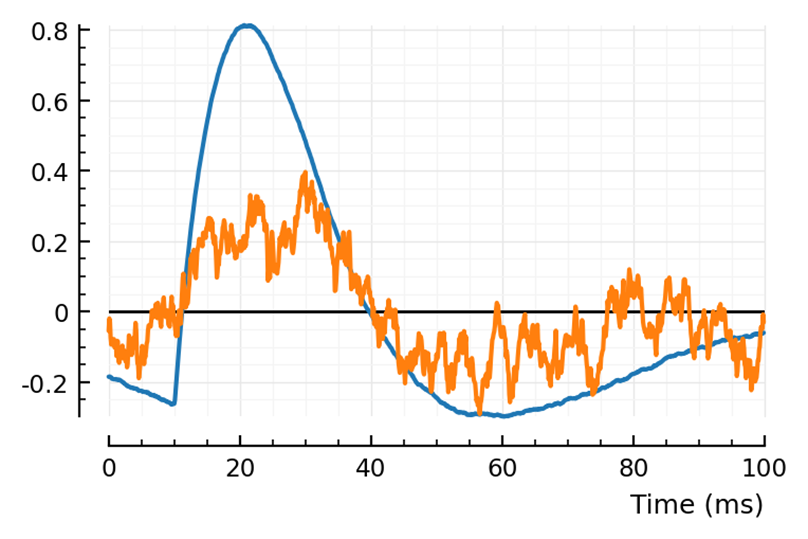
\includegraphics[w=1.15]{corr-overlay}
%     \captionof{figure}{An actual STA (orange), and the template it is correlated with (blue).}
%     \label{fig:corr-overlay}
% }

\begin{figure}
    \subfloat{
        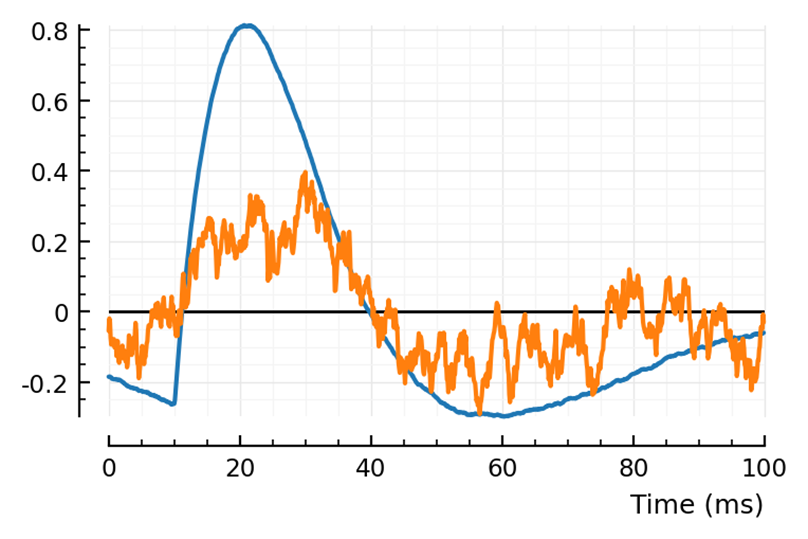
\includegraphics[w=0.7]{corr-overlay.png}
        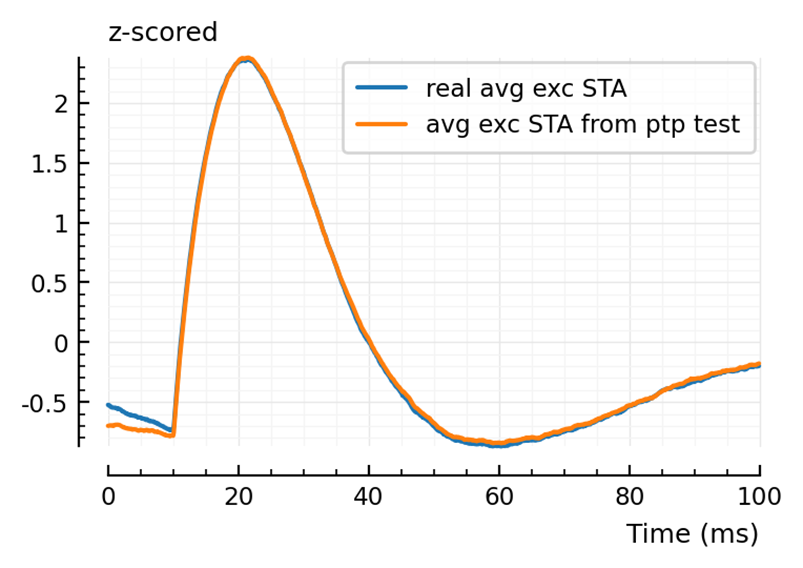
\includegraphics[w=0.7]{corr2.png}
    }
    \captionn[. ]
    {Correlating the STA with a template}
    {\Left: An example STA, and the template it will be correlated with to calculate the connection test statistic.\\
    \Right: Two possible STA templates: in blue, the average of the STAs of many true excitatory connections (namely of 50 neurons -- part of a 1000-neuron recurrent network -- that all had their voltage recorded; and all their excitatory inputs).
    In orange, the average STA of the excitatory connections detected with a strict `peak-to-peak' test.}
    \label{fig:corr}
\end{figure}

We find that this correlation-based test statistic outperforms the simple peak-to-peak measure (\cref{fig:N_sweep__AUC__template-corr_vs_STA}).

\begin{figure}
    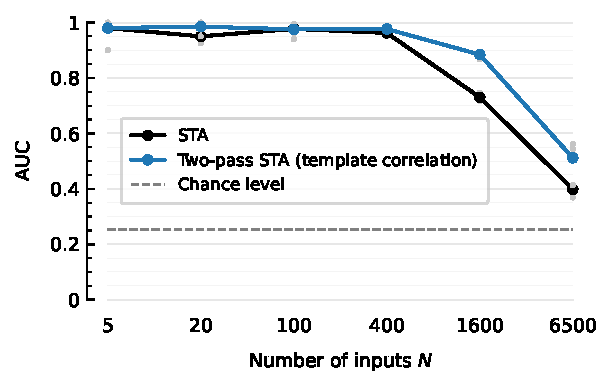
\includegraphics{perf-all-inputs__template-cor}
    \captionn
    {Correlation outperforms STA height as connection test}
    {Compare also with \cref{fig:N_sweep__AUC__upstroke_vs_STA}.\\
    AdEx neuron, 10-minute recording, no voltage imaging noise,  5 different seeds (blue dots). All $N$ inputs are tested (instead of just the highest firing ones), in addition to $N$ random unconnected spiketrains. AUC chance level is at $0.252$ (as in \cref{fig:AUC_chance_level}).\\
    Source: \nburl{2024-05-26__Fix_template-based_method}.}
    \label{fig:N_sweep__AUC__template-corr_vs_STA}
\end{figure}





\clearpage
\FloatBarrier
\section{Fitting a full STA model}
\label{sec:fitting-a-full-STA-model}

% \begin{itemize}
%     \item Model design
%     \item Iterative model fitting
%     \item Problem of overfitting, and parameter-constraints to solve it
%     \item An advantage: fit parameters (like transmission delay and time constants) are biologically ~meaningful
%     \item Perfomance for different N, \& comparison with previous methods
% \end{itemize}

Instead of a data-driven approach for the `ideal' STA shape, for this method we manually design a function (a 7-parameter function that we'll call $f$), which we will fit to the actual STAs.

\marginpar{
    \vspace*{-5em}
    \hspace*{-1.6em}
    \begin{tikzpicture}
    \begin{axis} [
        width = 7cm,
        height = 4cm,
        axis line style = {draw = none},
        grid = major,
        tick style = {draw = none},
        xtick = {0, 10},
        ytick = {0, 1/e},
        % ymajorticks = false,
        xlabel = {$t$} ,
        xlabel shift = {-14pt},
        ticklabel style = {font=\small, color = LighterBlack},
    ]
        \addplot [ultra thick, domain = 0:10, samples=400]
            {x * exp(-x)}  % max is 1/e, at t = 1.
            [yshift=26pt] node [pos = 0.4] {$t \, e^{-t}$};
    \end{axis}
\end{tikzpicture}

    \captionof{figure}{\small A simple PSP model.}
    \label{fig:alpha-function}
    \vspace*{2em}
}

One part of this STA model function is shaped like a postsynaptic potential bump (PSP, \cref{fig:alpha-function}). It is the impulse response of two linear integrators placed in series. Or, in other words, the convolution of two `step-and-decay' functions.\footnote{
    `Step-and-exponential-decay': $u(t) · e^{–t/τ}$, with $u(t)$ the Heaviside step function $\bm{1}_{t ≥ 0}$.
}%
$^{,}$  % comma between footnotemarks
\footnoteatfoot{
        In computational neuroscience, this function is sometimes called the `alpha function' or `alpha synapse'. \emph{Synapse}, because the double integrator model can be used to model synaptic conductance ($g$), with then a fast rise τ₁ (modelling neurotransmitter release), and a slower decay τ₂ (modelling its dissipation). The synaptic conductance model in our simulation is simpler: the `rise' is instant, i.e. we only have exponential decay.
}
It is the postsynaptic potential in the simplest linear neuron model ($\d{v} · τₘ = -v + I$) where the synaptic current $I$ is also linear ($\d{I} · τₛ = -I + s$).\footnote{
    $τₛ$ and $τₘ$ are the synaptic and membrane time constants, and
    $s(t) = \sumᵢ δ(t - tᵢ)$ is the train of input spikes $i$.
}

Solving for $v$ and with a single input spike at $t = 0$, we have, for $t ≥ 0$:
\begin{equation}
    \text{PSP}(t) = \begin{cases}
        t\, e^{-t/τₘ}   &\hspace{8pt} τₘ = τₛ \\
        \frac{τₘτₛ}{τₘ–τₛ} \left( e^{–t/τₘ} – e^{–t/τₛ} \right)  &\hspace{8pt} τₘ ≠ τₛ
    \end{cases}
    \label{eq:PSP}
\end{equation}

We find that this function approximates the shape of the \emph{simulated} postsynaptic potential in our actual neuron model well  -- even though our neuron model is not so linear.\footnote
    {Our model for the membrane potential has a component (the adaptation current $u$) whose differential equation recurrently depends on $v$. Additionally, the synaptic currents $Iⱼ$ are \emph{conductance-based}, meaning that they also recurrently depend on $v$: $Iⱼ = gⱼ \, (v – Eⱼ)$ (with $Eⱼ$ the reversal potential at synapse $j$, and the synaptic conductance $gⱼ$ a linear integrator of the input spike train $sⱼ(t)$:\newline
    $\d{gⱼ} · τ_{s,j} = – gⱼ + sⱼ$).}

But even though \cref{eq:PSP} models our simulated \emph{PSPs} well, it does not resemble our \emph{STAs}\footnote{
    This falsifies our initial implicit hypothesis that STAs are merely noisy reflections of PSPs.
};
see for example the average STAs in \cref{fig:corr}.
First, the bump in the STA does not occur immediately after the presynaptic neuron's spike. This is due to the simulated axonal transmission delay, and it is easily replicated in the model by shifting the PSP function in time. But more interestingly, the STA shows a sort of `dip', where it dives below baseline just after the PSP bump, and flares up again at the ends (a downwards slant in the initial delay period, and an upwards slant at the end of the STA).\\
\Cref{fig:N_1_signals} from \cref{ch3-STA} gives a clue to the reason for this dip: when there are no poststynaptic spikes (second and fourth column in \cref{fig:N_1_signals}), there is also no dip visible in the STAs (second and third rows). This dip thus seems related to these postsynaptic spikes, maybe enhancing the PSP right before and during the spike, and suppressing it right after (when the voltage is reset).

\begin{figure}
    \subfloat{
        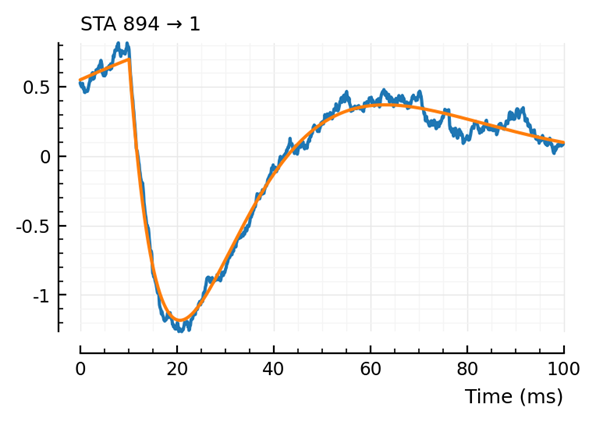
\includegraphics[w=0.66]{modelfit-overlay.png}
        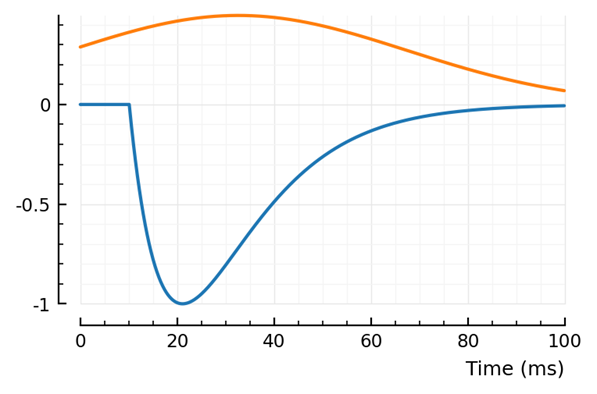
\includegraphics[w=0.66]{modelfit-components.png}
    }
    \captionn[. ]
    {Fitting a parametric model to the STA}
    {\Left: the model $f$ (orange) fit to the STA of an example inhibitory connection from a network simulation (blue). Both signals are z-scored.
    The components of the orange model function are shown on the
    \Right: the delayed simple PSP model (blue) and  the Gaussian `dip' (orange).}
    \label{fig:modelfit}
\end{figure}

The phenomena of the delay and the `dip' thus differentiate an STA from a PSP. We find empirically that the dip can be parsimonously modelled by subtracting a broad Gaussian curve from the PSP: see \cref{fig:modelfit}, right.\footnote{
    Note that in \cref{fig:modelfit}, we fit an \emph{inhibitory} STA, and the model componentes are thus inverted: the delayed PSP bump (blue) is downwards, and the Gaussian `dip' (orange) is upwards.
}

Our model $f$ is thus the difference of a delayed version of \cref{eq:PSP}, and a  Gaussian curve. The result is scaled by some factor α, to match the size of the specific STA that is being fit. α can be negative, to model inhibitory connections; $f$ is then flipped upside-down, as in \cref{fig:modelfit}.

The model function thus has seven parameters: the PSP's delay, $τₘ$, and $τₛ$; the Gaussian's location, width, and relative height wrt.~the PSP; and the final scaling α.
All parameters, except for the Gaussian's, have a ready biophysical interpration.\footnote
    {Namely: α is proportional to the connection strength, and indicates excitation (+) or inhibition (–). The PSP's delay, $τₘ$, and $τₛ$ are estimates of the axonal transmission delay and the synaptic and membrane time constants.}

We fit the model function to individual STAs using nonlinear least-squares optimization; more specifically using the Levenberg-Marquardt algorithm.\footnote{
    This is the standard method for nonlinear least-squares optimization. For example, in \textsc{Matlab}'s \texttt{lsqcurvefit} function,  it is the default algorithm when the number of functions (in our case, 1) exceeds the number of datapoints (in our case, 1000:  100 ms of signal post-spike, at Δt = 0.1 ms).\newline
    We used the Levenberg-Marquardt implementation of the Julia package \href{https://github.com/JuliaNLSolvers/LsqFit.jl}{LsqFit.jl}.
}
%
% To make this fitting procedure work well, three things had to be done.
To make the fitted functions well-behaved and looking like actual STAs, we had to limit the creative freedom of the optimization algorithm, by enforcing box constraints on the parameters.
% - decouple params
%  (https://tfiers.github.io/phd/nb/2022-09-13__Fit_simpler_function.html)
% - 100× speedup

The final test statistic is the mean squared error (MSE) between z-scored versions of the fitted function and the STA. The normalization by z-scoring is necessary to be able to compare goodness of fit between STAs with different ranges\footnote{
    Most importantly between a real STA and its shuffled versions.
    Because those shuffled STAs have a smaller range, they will have a lower MSE, even though the fit is visually clearly worse.
}

In comparison with the previous two methods (STA height and STA template correlation), this model-fitting approach did not perform significantly better than STA height, and it was clearly worse than template correlation.

The model-fitting is also very computationally expensive: iteratively fitting a nonlinear function to an STA takes much longer than simply calculating a Pearson correlation between two STA signals.

For these two reasons, we have not performed an extensive performance evaluation of this method, as we have done for the previous and following methods (\cref{fig:N_sweep__AUC__template-corr_vs_STA,fig:N_sweep__AUC__upstroke_vs_STA} respectively).

One advantage of this model-fitting method over the other methods though, is that most of the fitted parameters have a ready biophysical explanation: connection strength, transmission delay, and synaptic and membrane time constants.







% \begin{itemize}
%     \item Non-STA method: concatenated individual windows as (X, y)
%     \item Examples of pooled windows, and fits
%     \item Mention the problem of unknown transmission delays
%     \item Perfomance for different N, \& comparison with previous methods
% \end{itemize}

\clearpage
\section{Linear regression of the upstroke}

All previous methods are STA-based, i.e. different windows are cut from the postsynaptic voltage signal -- one window for every presynaptic spike -- and these are averaged into one signal, which is then used for further analysis. The method described in this section does not use STAs. We still construct the spike-triggered windows, but we do not average them. Instead, we use them to construct a gigantic data matrix for use in a linear regression.

Every single timepoint on the x-axis (in relative time after the presynaptic spike) will correspond to multiple voltage values on the y-axis; namely one for every window. Whereas for an STA, every timepoint on the x-axis corresponds to just a single y-value (the average voltage).

Why a linear regression? As we saw with the STAs in previous sections, they do not look like a line. But their first part, the "upstroke", might be approximated by one.

Let's number our spike-triggered windows $1, 2, .., N$ (for a presynaptic spiketrain with $N$ spikes), and let's number the voltage values in window $i$ as $[y_{i,1}, y_{i,2}, .., y_{i,M}]$ (for a window length of $M$ samples long).\footnote{
    This window length $M$ is an important parameter. The window must be approximately as long as the upstroke of the STA/PSP: not longer (so that the shape is too complex to be fit by a line), nor shorter (so that there would not be enough data for a proper fit).
}
We will then perform the following linear regression:
\begin{align}
    \bm{y} \hspace{1.4em}
    &=  \hspace{1.6em}
    X  \hspace{2.2em}
    \bm{β}  \hspace{0.7em}
    + \hspace{1.4em}
    \bm{ε}
    \\[1em]
    \begin{bmatrix}
        y_{1,1} \\
        y_{1,2} \\
        \vdots \\
        y_{1,M} \\
        y_{2,1} \\
        y_{2,2} \\
        \vdots \\
        \vdots \\
        y_{N,M}
    \end{bmatrix}
    &=
    \begin{bmatrix}
        1 & 1 \\
        1 & 2 \\
        \vdots & \vdots \\
        1 & M \\
        1 & 1 \\
        1 & 2 \\
        \vdots & \vdots \\
        \vdots & \vdots \\
        1 & M
    \end{bmatrix}
    \begin{bmatrix}
        β_0 \\
        β_1
    \end{bmatrix}
    +
    \begin{bmatrix}
        ε_{1,1} \\
        ε_{1,2} \\
        \vdots \\
        ε_{1,M} \\
        ε_{2,1} \\
        ε_{2,2} \\
        \vdots \\
        \vdots \\
        ε_{N,M}
    \end{bmatrix}
\end{align}
I.e. we will regress voltage-after-spike against time-after-spike.\\
Note that the noise term here is not just modelling the Gaussian noise we explicitly add ourselves (i.e. the voltage imaging noise); but rather \emph{everything} that is not the increase in the poststynaptic voltage due to a presynaptic spike. This is mainly the effects of other presynaptic neurons, and postsynaptic spikes.

If we assume additive Gaussian noise, i.e.
\begin{equation} \label{eq:sampling_noise}
    ε_{i,j} \sim \mathcal{N}(0, σ^2)
\end{equation}
then the maximum-likelihood estimate $\hat{\bm{β}}$ of the regression parameters $\bm{β}$ is obtained through minimizing the mean squared error (MSE)\footnote{
    \url{https://statproofbook.github.io/P/slr-mle}
}
between our observed voltage values $\bm{y}$ and the fitted line $\hat{\bm{y}} = X \hat{\bm{β}}$:
\begin{equation}
    \hat{\bm{β}} = \argmin_{\bm{β}} || \bm{y} - X \bm{β} ||_2^2.
\end{equation}
Our linear regression problem has become standard ordinary least squares (OLS) regression, for which a closed-form solution exists: the so-called normal equations,
\begin{equation} \label{eq:normal-eqs}
    \hat{\bm{β}} = (X^T X)^{-1} X^T \bm{y}
\end{equation}
As is standard practice and for numerical stability ("don't explicitly invert a matrix if not needed"), we instead find the optimal intercept ($\hat{β}_0$) and slope ($\hat{β}_1$) of our linear fit using QR-factorization, via Julia's left-division operator: \texttt{$\hat{\bm{β}}$ = X \textbackslash \ y}.

From this linear fit we thus obtain a slope $\hat{β}_1$. To use our regression as a connection test, we will perform a hypothesis test on this slope. The null hypothesis is that this slope is zero ($H_0: \hat{β} = 0$): the voltage of the tested neuron does not react to spikes of the other tested neuron, and on average it stays flat.

If the slope $β_1$ really were $0$, then we would expect the fitted slope $\hat{β}_1$ to be distributed normally around $0$, as follows:\footnote{
    \url{https://gregorygundersen.com/blog/2021/09/09/ols-hypothesis-testing/}
}
\begin{equation} \label{eq:slope_distrib}
    \hat{β}_1 \sim \mathcal{N}(0, σ^2 [Q]_{2,2})
\end{equation}
where $σ^2$ is the variance of the sampling noise (\cref{eq:sampling_noise}), and $[Q]_{2,2}$ is the second diagonal element of the 'cofactor matrix' $Q$,\footnote{
    The indices are off by one ($\hat{β}_1$ vs $[Q]_{2,2}$), because the intercept in linear regression is conventionally called $β_0$, and so we start numbering the elements of $\bm{β}$ from $0$; but we number the elements of other vectors/matrices from $1$.
}
which is the inverse of the Gram matrix $X^T X$:
\begin{equation}
    Q = (X^T X)^{-1}
\end{equation}

We do not know what the sampling noise $σ^2$ is, but we have a maximum-likelihood estimate $\hat{σ}^2$ for it,\footnote{\url{https://statproofbook.github.io/P/slr-mle}} namely the mean squared error (MSE) of the fit:
\begin{equation}\label{eq:σhat}
    \hat{σ}^2 = \frac{1}{n} || \bm{y} - X \bm{\hat{β}} ||_2^2
\end{equation}
(where $n = M · N$ is the number of datapoints).

Our final test statistic $t$ to determine whether there is a connection from neuron A
to neuron B is then the slope of the fit (of B's voltage after neuron A's spikes), normalized by how noisy the parameter fit is:
\begin{equation} \label{eq:linreg-tstat}
    t = \hat{β}_1 / \hat{σ}_{\hat{β}_1}
\end{equation}
where $\hat{σ}_{\hat{β}_1}$ is the standard error of the slope (\cref{eq:slope_distrib} with \cref{eq:σhat}):
\begin{equation} \label{eq:linreg-stderr-β}
    \hat{σ}_{\hat{β}_1} = \sqrt{\hat{σ}^2 [Q]_{2,2}}
\end{equation}

Unlike in \cref{eq:slope_distrib}, $t$ is no longer strictly normally distributed.\footnote{
    Instead, it follows a Student's $t$-distribution, with $n - p$ degrees of freedom, where $n = M · N$ is the number of datapoints, and $p = 2$ is the number of parameters of the regression ($β_0$ and $β_1$).
}
But when the number of datapoints is quite large, as is the case here, the $t$-distribution becomes practically normal, and our test statistic $t$ will very closely follow the standard normal distribution under the null hypothesis ("the slope is zero").

We can (and do) use this $t$-value as-is in our connection test, i.e. as the test statistic over which the detection threshold is swept.

Additionally, if our assumptions (linear data-generating process, additive Gaussian noise) would be correct,\footnote{They are not. As one example, consider postsynaptic spikes as one of the sources of noise on the PSP: they are assymetrical (spikes are always upwards, never downwards). \Cref{fig:linefit-residuals} shows that the residuals of a linear regression of an example STA are not symmetric.}
we could also assign an actual probability (a $p$-value) to observing slopes as extreme as observed. Because $t$ follows the standard normal distribution under the null-hypothesis, and with $\phi(x)$ the cumulative probability function of this distribution, we have: $p = 2\ \phi(-|t|)$: the probability that a sample smaller than $-|t|$ or larger than $|t|$ is drawn.

As seen in \cref{fig:linefit-residuals}, our assumption of additive Gaussian noise $ε$ on the regression does not seem valid. But our goal for this regression was not to build a statistical model of the STA, but rather to use the fit as a tool for connection detection, something at which it is empirically succeeds, notwithstanding the violated statistical assumptions.

% \footnote{
%     Besides the maximum-likelihood estimator $\hat{σ}^2$, there is also a Bessel-corrected estimator of $σ^2$, namely $s^2 = \frac{n}{n-p} \hat{σ}^2$ (with $p = 2$ the number of parameters in the regression). Unlike $\hat{σ}^2$, this is an unbiased estimator ($\mathbb{E}[s^2] = σ^2$); "but it has a higher MSE".
% }

\Cref{fig:N_sweep__AUC__upstroke_vs_STA} shows the performance of the described linear regression method, for different number of inputs $N$, and compared to the STA height method. We find a perfect performance (AUC of $1$) for up to $400$ inputs. After that, the AUC starts to drop, but it stays much higher than the STA height method. At the realistic number of inputs $N = 6500$, the linear fit's AUC is still at $0.5$, while the STA height method performs at chance level ($≈ 0.25$)

\begin{figure}
    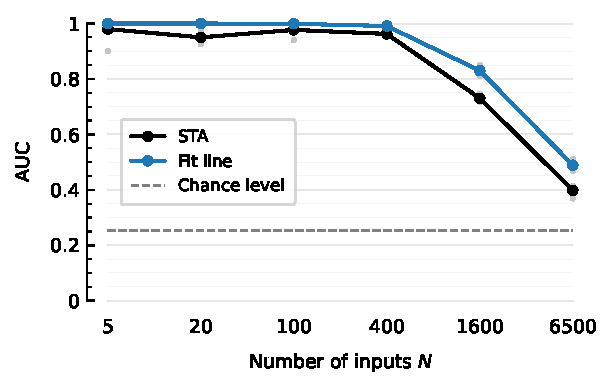
\includegraphics{perf-all-inputs__fitline.pdf}
    \captionn
        {Line fit outperforms STA height as connection test}
        {AdEx neuron, 10-minute recording, no voltage imaging noise,  5 different seeds (blue dots). All $N$ inputs are tested (instead of just the highest firing ones), in addition to $N$ random unconnected spiketrains. AUC chance level is at $0.252$ (as in \cref{fig:AUC_chance_level}). \\
        Source: \nburl{2024-05-26__Fix_template-based_method}.}
    \label{fig:N_sweep__AUC__upstroke_vs_STA}
\end{figure}



\begin{figure}
    \subfloat{
        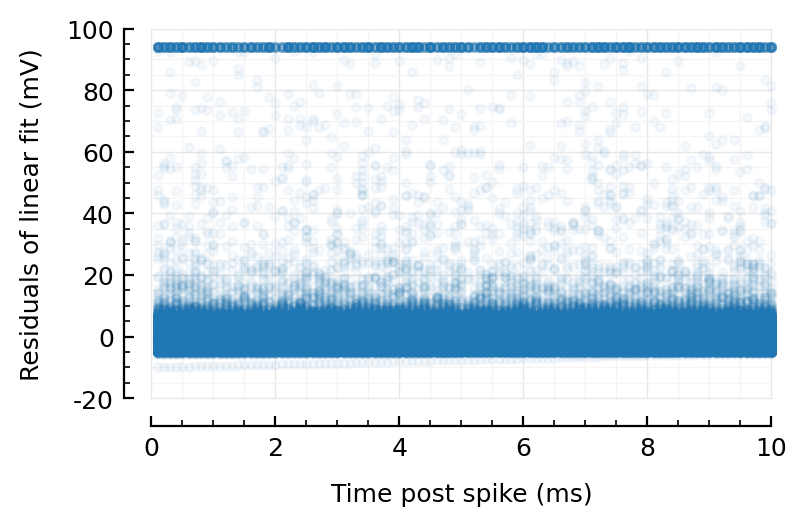
\includegraphics[w=0.7]{residuals_vs_time.png}
        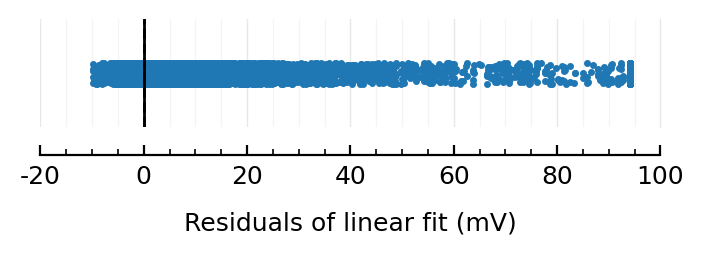
\includegraphics[w=0.7]{residuals_distplot.png}
    }
    \captionn
        {Residuals of an example regression}
        {
        Linear regression of the first 10 ms of the spike-triggered average voltage of an AdEx neuron with 6500 inputs simulated for 10 minutees, for its highest-firing excitatory input.
        Left: Residuals over time.
        Right: Distribution of residuals marginalized over time; vertical black line indicates both the mean ($-5.9 × 10^{-12}$~mV) and the median ($0.1$~mV).\\
        The residuals seem to be homoskedastic, but are not symmetrically distributed.\\
        Source: \nburl{2024-05-29__Residuals-linefit}.
        }
    \label{fig:linefit-residuals}
\end{figure}


% This section can go to Appendix.
\subsection{Relationship to fitting the STA}

For this last method, we emphasized that it does not operate on the STA, but instead uses the individual windows directly. But an analysis of the normal equations (\cref{eq:normal-eqs}) reveals that fitting a line to all the individual windows pooled together is actually very similar to fitting a line to their average, the STA.

The linear regression on the STA has the following response vector $\overline{\bm{y}}$ and design matrix $\overline{X}$:
\begin{align}
    \overline{\bm{y}} \hspace{6em}
    &=  \hspace{1.6em}
    \overline{X}  \hspace{2.2em}
    \overline{\bm{β}}  \hspace{0.7em}
    + \hspace{1.4em}
    \overline{\bm{ε}}
    \\[1em]
    \frac{1}{N}
    \begin{bmatrix}
        y_{1,1} + y_{2,1} + … + y_{N,1} \\
        y_{1,2} + y_{2,2} + … + y_{N,2} \\
        \vdots \\
        y_{1,M} + y_{2,M} + … + y_{N,M}
    \end{bmatrix}
    &=
    \begin{bmatrix}
        1 & 1 \\
        1 & 2 \\
        \vdots & \vdots \\
        1 & M
    \end{bmatrix}
    \begin{bmatrix}
        β_0 \\
        β_1
    \end{bmatrix}
    +
    \begin{bmatrix}
        ε_1 \\
        ε_2 \\
        \vdots \\
        ε_M
    \end{bmatrix}
\end{align}

We see that the previous design matrix $X$ consists of $N$ stacked repetitions of the design matrix $\overline{X}$ here.

We can show that both regressions have the same solution for their normal equations, i.e. that
\begin{align} \label{eq:normal-eqs-equivalent}
\begin{split}
    \hat{\bm{β}}
    &= (X^T X)^{-1} X^T \bm{y} \\
    = \hat{\overline{\bm{β}}}
    & = (\overline{X}^T \overline{X})^{-1} \overline{X}^T \overline{\bm{y}}
\end{split}
\end{align}

As an example, working out the second element of $X^T \bm{y}$, we find:
\begin{align}
    [X^T \bm{y}]_2
    &= [1\ 2\ … M] · \bm{y_1} + [1\ 2\ … M] · \bm{y_2} + … + [1\ 2\ … M] · \bm{y_N}  \nonumber \\
    &= [1\ 2\ … M] · (\bm{y_1} + \bm{y_2} + … + \bm{y_N})   \nonumber \\
    &= [1\ 2\ … M] · N \overline{\bm{y}}   \nonumber \\
    &= N · [\overline{X}^T \overline{\bm{y}}]_2
\end{align}
(where $·$ is the inner or dot product, and $\bm{y_i} = [y_{i,1}\ y_{i,2}\ …\ y_{i,M}]$).

The same is true for the first element of $X^T \bm{y}$ (just with $[1\ 1\ …\ 1]$ instead of $[1\ 2\ …\ M]$), so that
\begin{equation} \label{eq:XTy-eq}
    X^T \bm{y} = N · \overline{X}^T \overline{\bm{y}}
\end{equation}

A similar argument can be made for each of the four elements of the Gram matrix, and we find that $X^T X = N · \overline{X}^T \overline{X}$.\\
That makes the cofactor matrix:
\begin{equation} \label{eq:Q-eq}
    (X^T X)^{-1} = \frac{1}{N} (\overline{X}^T \overline{X})^{-1}
\end{equation}
Taking together \cref{eq:XTy-eq,eq:Q-eq}, we indeed find the exact same solutions $\hat{\bm{β}}$ for the line fit (\cref{eq:normal-eqs-equivalent}), whether regressing all individual windows, or their average.

Even though the fitted slope $\hat{β}_1$ is the same, there is a difference in its standard error (\cref{eq:linreg-stderr-β}), and thus also in the test statistic $t$ we'd use as a connection test (\cref{eq:linreg-tstat}).\\
We can write the standard error on the slope in the first regression (on all the individual windows) as follows:\footnote{
    where $c$ is shorthand for $\sqrt{\left[\overline{Q}\right]_{2,2} / M}$.
}
\begin{align}
    \hat{σ}_{\hat{β}_1}
    &= \frac{1}{N}\ c\ || \bm{y} - X \hat{β} ||_2  \\
    &= \frac{1}{\sqrt{N}}\ c\ \sqrt{\sum_{j=1}^M \frac{1}{N}\sum_{i=1}^N
    \left( y_{i,j} - (\hat{β}_0 + \hat{β}_1 · j)  \right)^2 }  \label{eq:stderr-wins}
\end{align}

For the regression of the STA, we have:
\begin{align}
    \hat{σ}_{\hat{\overline{β}}_1}
    &= c\ || \overline{\bm{y}} - \overline{X} \hat{β} || _2 \\
    &=  c\ \sqrt{\sum_{j=1}^M \left(
        \left(\frac{1}{N}\sum_{i=1}^N y_{i,j}\right)
        - (\hat{β}_0 + \hat{β}_1 · j)  \right)^2 }   \label{eq:stderr-STA}
\end{align}

In other words, the standard error of the STA regression uses the squared error between the fitted line and the average measured voltage, whereas for the regression on all windows, we use the average of the squared errors between the fitted line and all of the individual measured voltages in one timepoint.

These last equations show the advantage of regression with individual windows, versus regressing the STA: the more windows are used (higher $N$) -- i.e. the more presynaptic spikes this possible connection has -- the lower the standard error on the fitted slope will be, and the higher the test statistic $t = \hat{β}_1 / \hat{σ}_{\hat{β}_1}$. This is thanks to the scaling by $1 / \sqrt{N}$ in \cref{eq:stderr-wins}, which is absent in \cref{eq:stderr-STA}.

This is a quantification of a heuristic that could go something like: ``the more `presynaptic' spikes there are, the more certain we can say there is or isn't a connection here''.\footnote{
    E.g, if two possible connections would have the same fitted slope for their spike-triggered voltages, but one of them has more presynaptic spikes, then that connection would have a higher test statistic, and would be favoured when classifying the connections.
} And when using just the STA, the knowledge of how many windows were used to calculate it is lost.

Two notes here: first, as the fitted parameters $\bm{β}$ are the same when regressing either all windows or the STA, we could just use the STA for fitting, and then manually add a correction factor $1 / \sqrt{N}$ to the test statistic $t$. This is interesting computationally, as you then don't have to construct the very long design matrix $X$ and response vector $\bm{y}$.\\
Second, one could argue the standard error of the STA regression \emph{does} already account for the number of windows used: the more windows are averaged together, the less the STA will be noisy and the more it will look like a straight line (at its upstroke portion at least); and the lower the standard error will be. Under this view, an additional correction factor in the test statistic to explicitly account for the number of windows / presynaptic spikes, is not necessary.




% \section{Clustering, \& Hierarchical model fitting}

% \begin{itemize}
%     \item (Time-permitting)
% \end{itemize}




% \section{Zhou/Cai's `Spike-triggered regression'}

% \begin{itemize}
%     \item (Time-permitting)
% \end{itemize}




% \section{Computational cost}

% \begin{itemize}
%     \item Timings of each method, extrapolation for larger number of tested connections
% \end{itemize}



% \begin{itemize}
%     \item Conclusions of the N-to-1 experiment
%     \item Leadup to the network experiments: what we could not yet test (the problem of indirect connections, as e.g. identified in the connectomics challenge)
% \end{itemize}

\clearpage
\section{Conclusion}

In this chapter we wondered whether we could improve upon the most obvious voltage-based connection detection method (namely measuring the height of the STA). We developed and tested three new methods. We found that two of them -- template correlation and linear regression of the upstroke -- indeed performed significantly better as a connection test. The third method we developed (fitting a parametric model to the STA shape) did not perform better as a connection test, but it does provide a method to estimate biophysical parameters of a connection.
